\section{Architecture of the System}
\phantomsection
\subsection{UML Diagrams}
The Unified Modeling Language (UML)\cite{uml} is a development and all use modeling language in the field of software engineering. Is indended to assure a standard way of visualizing the design of the system that it was made for.

In the current chapter is represented and described the architecture of Kyno application. It contains a set of relevant diagrams modeled in UML language. The diagrams provide a fundamental documentation an description of the system structure and behavior.

\begin{itemize}
\item Use Case Diagram;
\item Deployment Diagram;
\item Class Diagram
\item Sequence Diagram;
\item Activity Diagram;
\item State Diagram.

\end{itemize}
These diagrams will illustrate the users possibilities, the system architecture and will also illustrate the procedures of interaction between the modules.

\subsubsection{Use Case Diagram}
To model a system the most important aspect is to capture the dynamic behaviour. In UML there are five diagrams available to model dynamic nature and use case diagram is one of them. Now as we have to discuss that the use case diagram is dynamic in nature there should be some internal or external factors for making the interaction.

These internal and external agents are known as actors. So use case diagrams are consists of actors, use cases and their relationships. The diagram is used to model the system/subsystem of an application. A single use case diagram captures a particular functionality of a system.

So to model the entire system n numbers of use case diagrams are used.

Purpose of Use Case diagram is:

\begin{itemize}
\item Used to gather requirements of a system.
\item Identify external and internal factors influencing the system.
\item Show the interacting among the requirements are actors.
\item Used to get an outside view of a system.

\end{itemize}
\vspace{0.2cm}


In the \mbox{figure \ref{uc_general}} , is shown the process of the user that interacts with the application. Therefore 2 use case diagrams were modeled to show the set of avaiable actiones offered to the user's. The client part of the application represents an executable. As we can see the most important stages of the project is around  user's exercises, later in \mbox{figure} \ref{uc_exercise} we will see the type of exercises the user can do. The possibility of giving feedback to the application is offered. Also, the user can view the results after the end of the exercise or at the moment of doing the exercise.


\begin{figure}[!h]
\centering
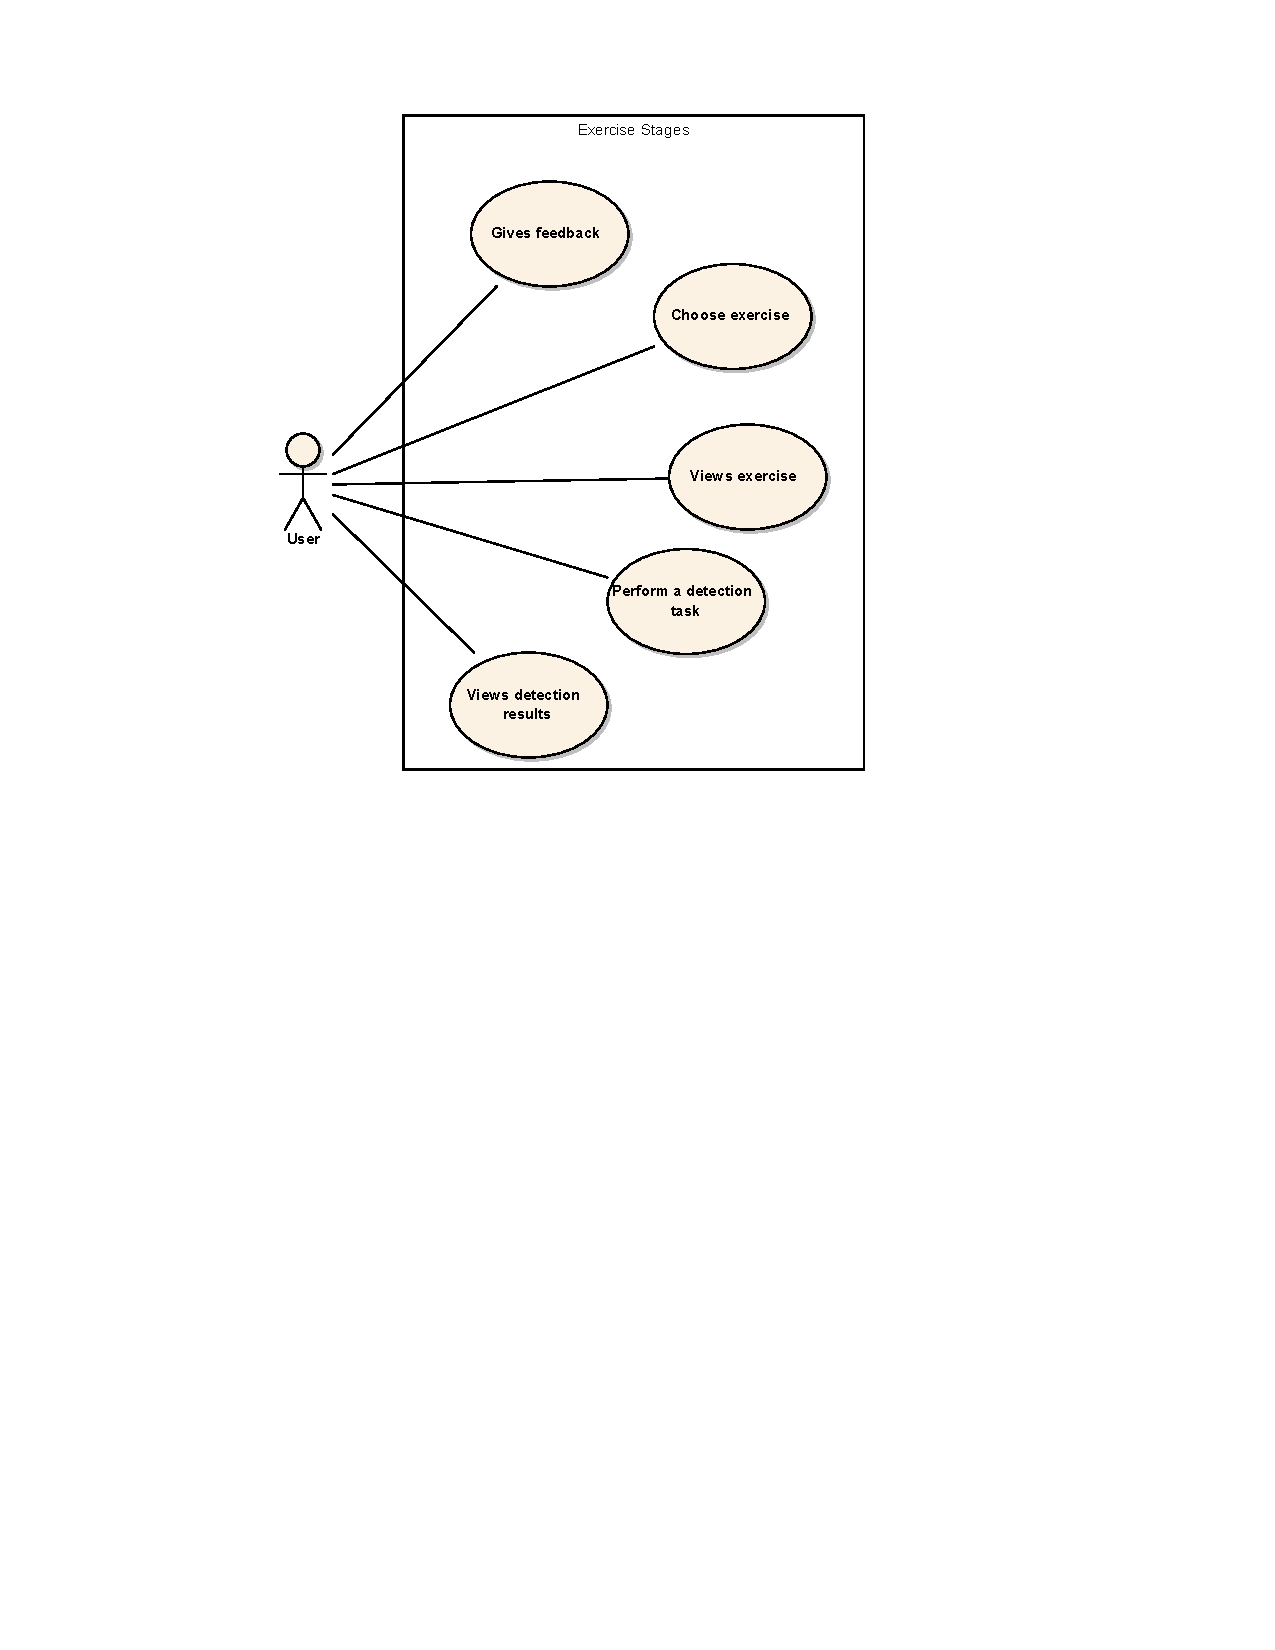
\includegraphics[trim={0 14.5cm 0 1cm},clip, width = 16cm]{2_uc_general}
\caption{General Use Case diagram of the system.}\label{uc_general}
\end{figure}

Now back to the \mbox{figure} \ref{uc_exercise} where the operations can be seen, there are 4 main actions an user can perform. When the user opens the application he will be provided with a menu he can choose one of this 4 actions from there. By choosing the first action which is grab the user will have to open and close slowly his hand n times. The second action is pinch, this action is a little bit more complicated since it will make the user to touch every finger, one after one, with the thumb. Next action and the third one is rotate. Rotate is rather simple, the user will have to rotate his hand horizontally untill its reaching the position of completing one rotation. The forth and the last action is movement, its not that complicated, just moving the hand from left to right and right to left will be counted as 1 movement. A text panel with results and a second panel with tips will be displayed on the screen for the user on each active action.


\begin{figure}[!h]
\centering
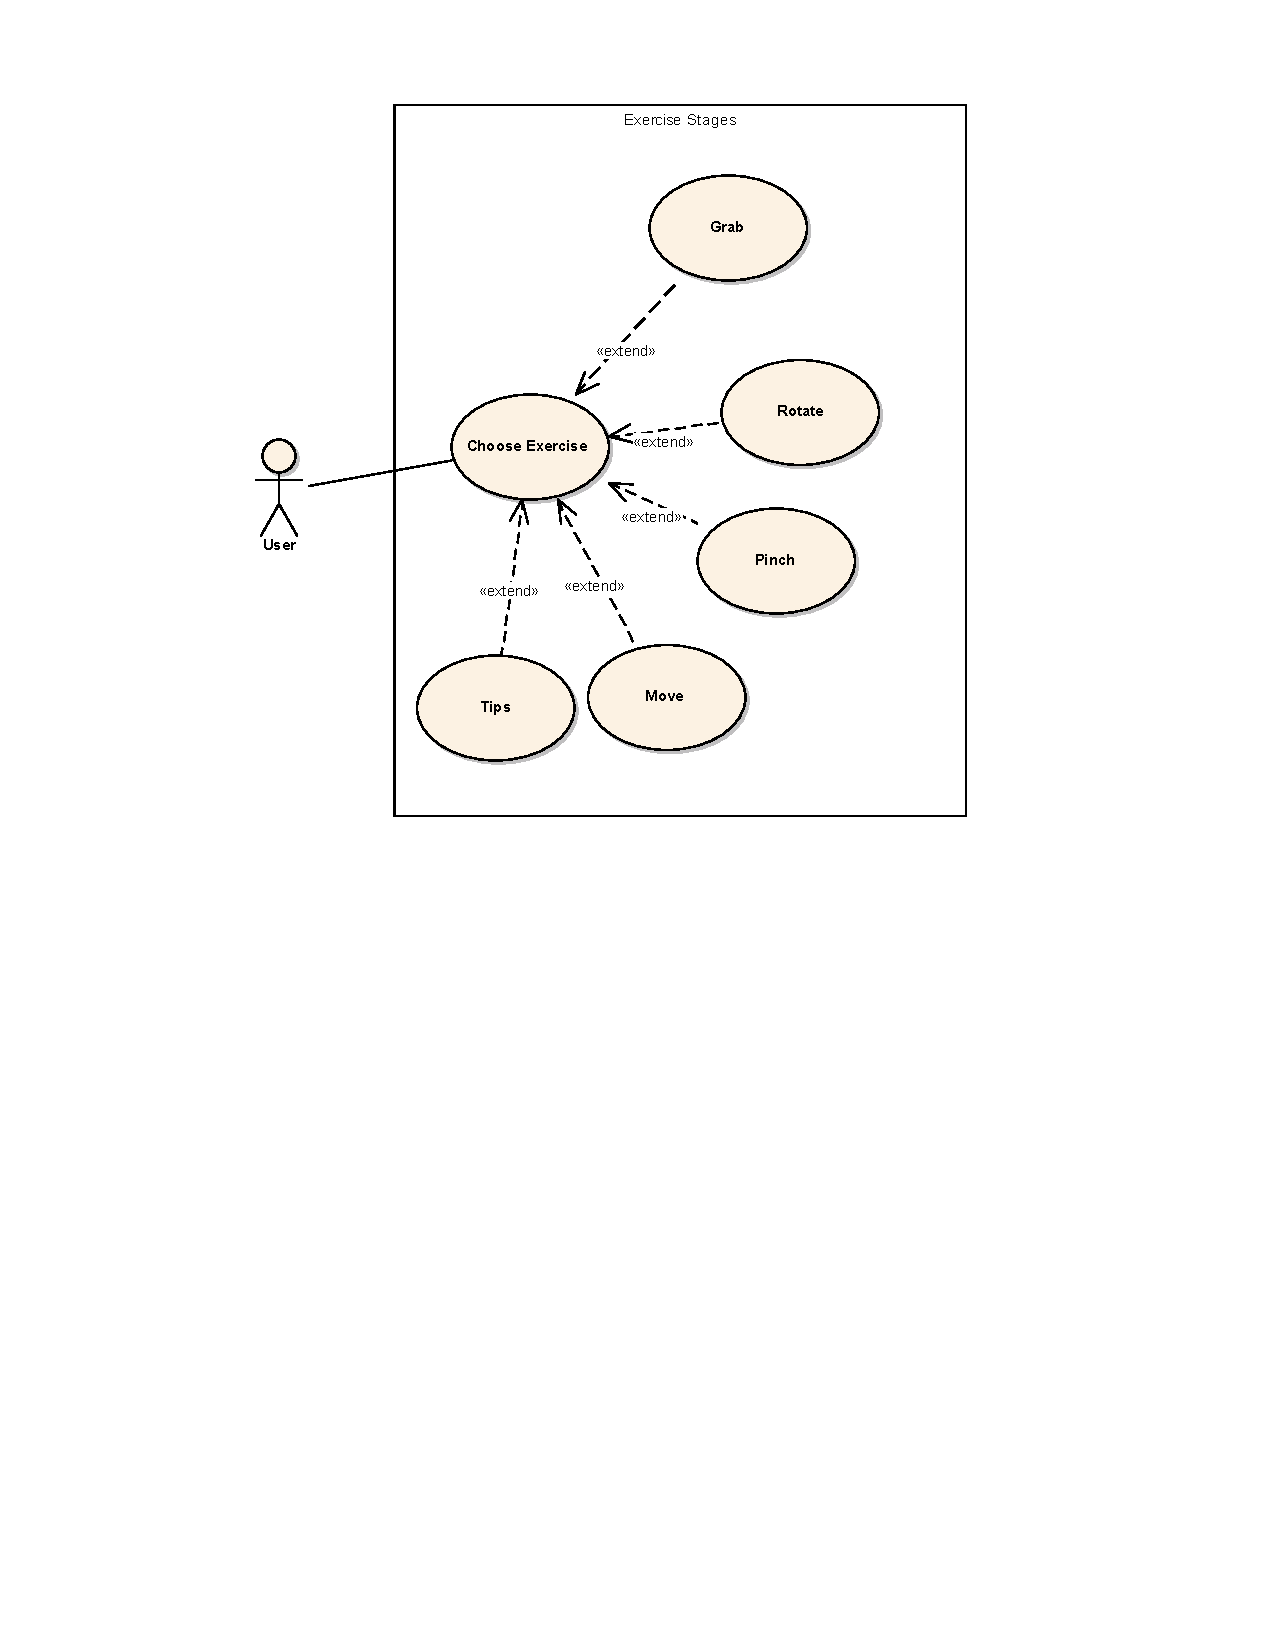
\includegraphics[trim={0 14cm 0 1cm},clip, width = 16cm]{1_uc_exercise_stage}
\caption{Use Case diagram of exercise action.}\label{uc_exercise}
\end{figure}



\subsubsection{Deployment Diagram}
Deployment diagrams are used to visualize the topology of the physical components of a system where the software components are deployed.

So deployment diagrams are used to describe the static deployment view of a system. Deployment diagrams consist of nodes and their relationships.

The purpose of deployment diagrams can be described as:
\begin{itemize}
\item Describe runtime processing nodes.
\item Describe the hardware components used to deploy software components.
\item Visualize hardware topology of a system.
\end{itemize}

\vspace{0.2cm}


\begin{figure}[!h]
\centering
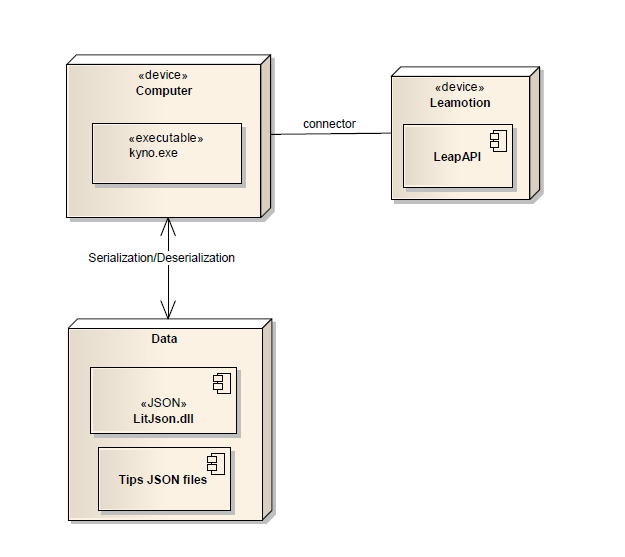
\includegraphics[trim={0 15.5cm 0 2cm},clip, width = 16cm]{1_deploy_diagram}
\caption{Deploy diagram of the system.}\label{deploy_diagram}
\end{figure}

\clearpage

\subsubsection{Class Diagram}
The class diagram is a static diagram and itrepresents the static view of an application. Describes the attributes and operations of a class and more than that, also the constraints appointed on the system.
Because class diagrams are the only UML diagrams that can be mapped directly with object oriented languages it is widely used in the modelling of the object oriented system and at the time of system construction.

Purpose of the class diagram can be summarized in:

\begin{itemize}
\item Analysis and design of the static view of an application.
\item Describe responsibilities of a system.
\item Base for component and deployment diagrams.
\item Forward and reverse engineering.
\end{itemize}

\vspace{0.2cm}



\begin{figure}[!h]
\centering
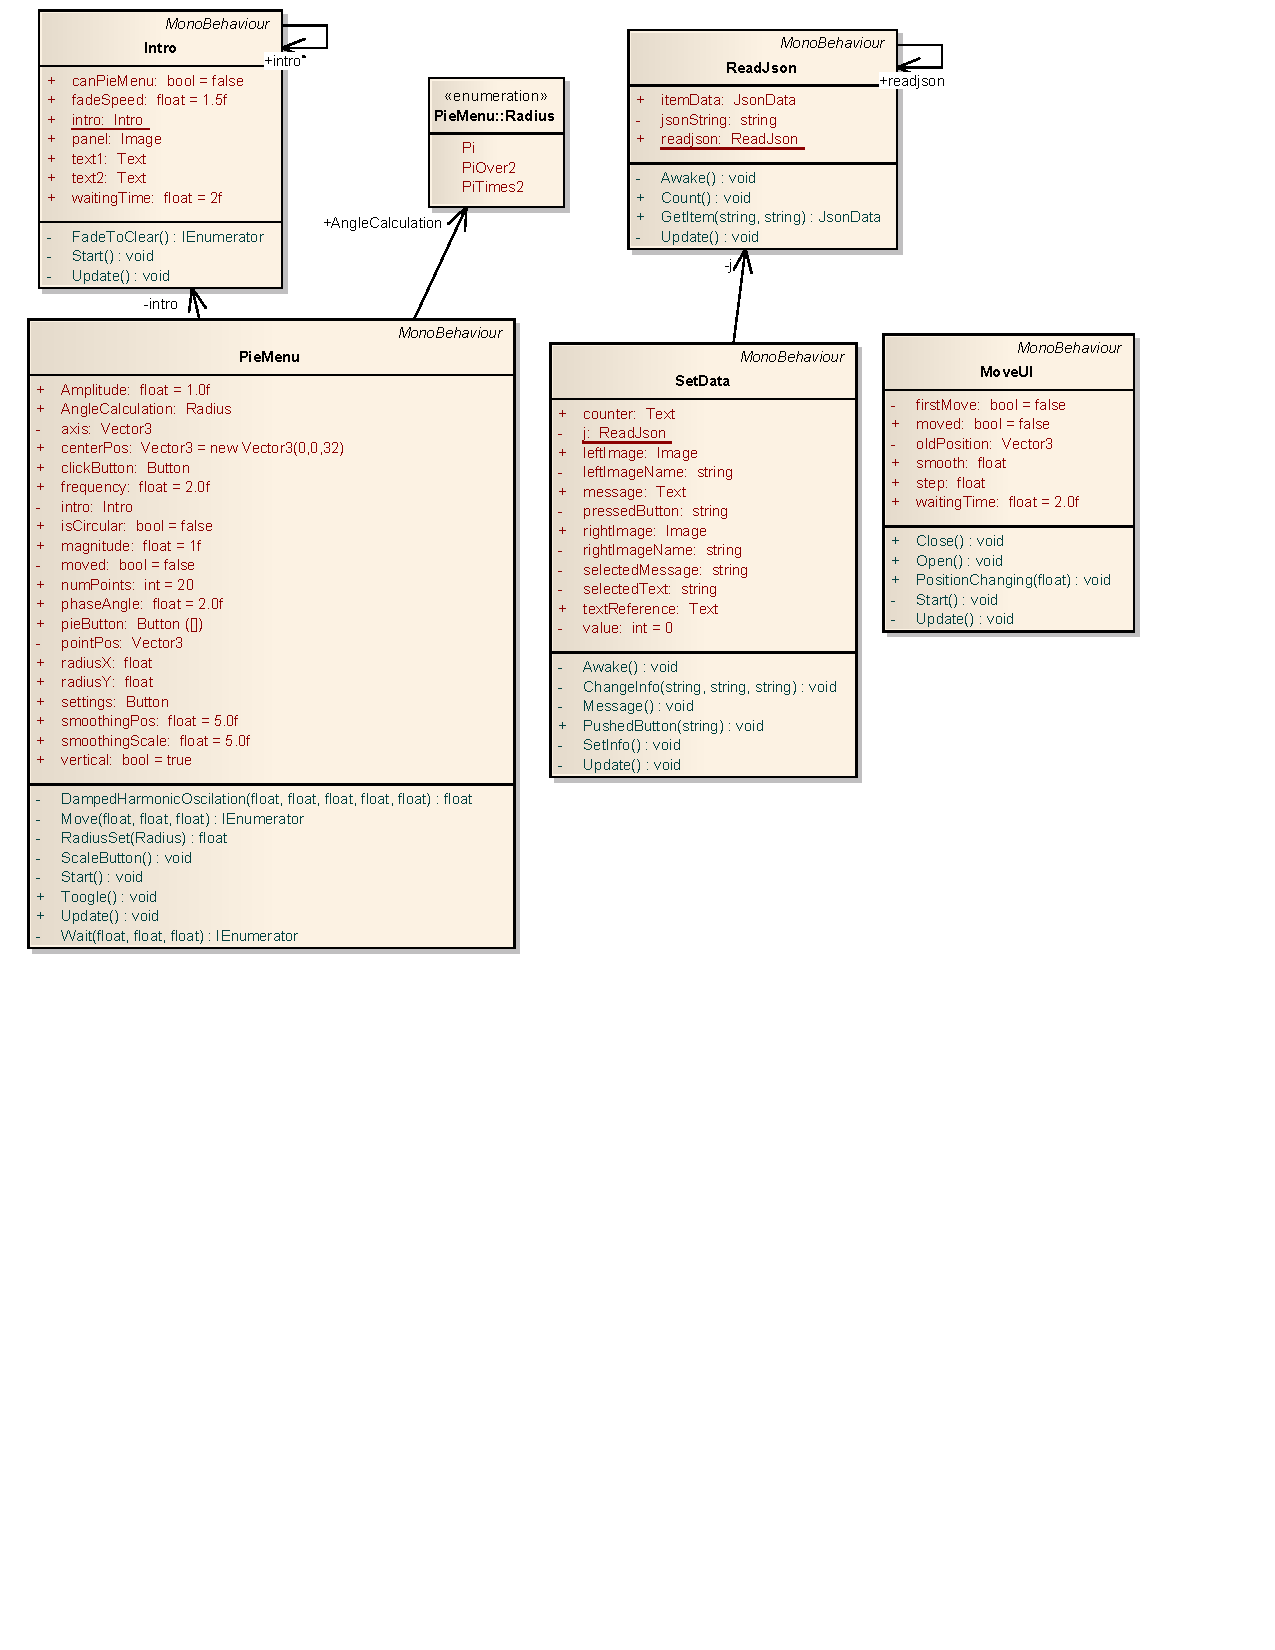
\includegraphics[trim={0 8cm 0 0cm},clip, width=16cm]{1_class_ui}
\caption{Class Diagram of User Interface and User Interaction.}\label{class_ui}
\end{figure}

\clearpage

\begin{figure}[!h]
\centering
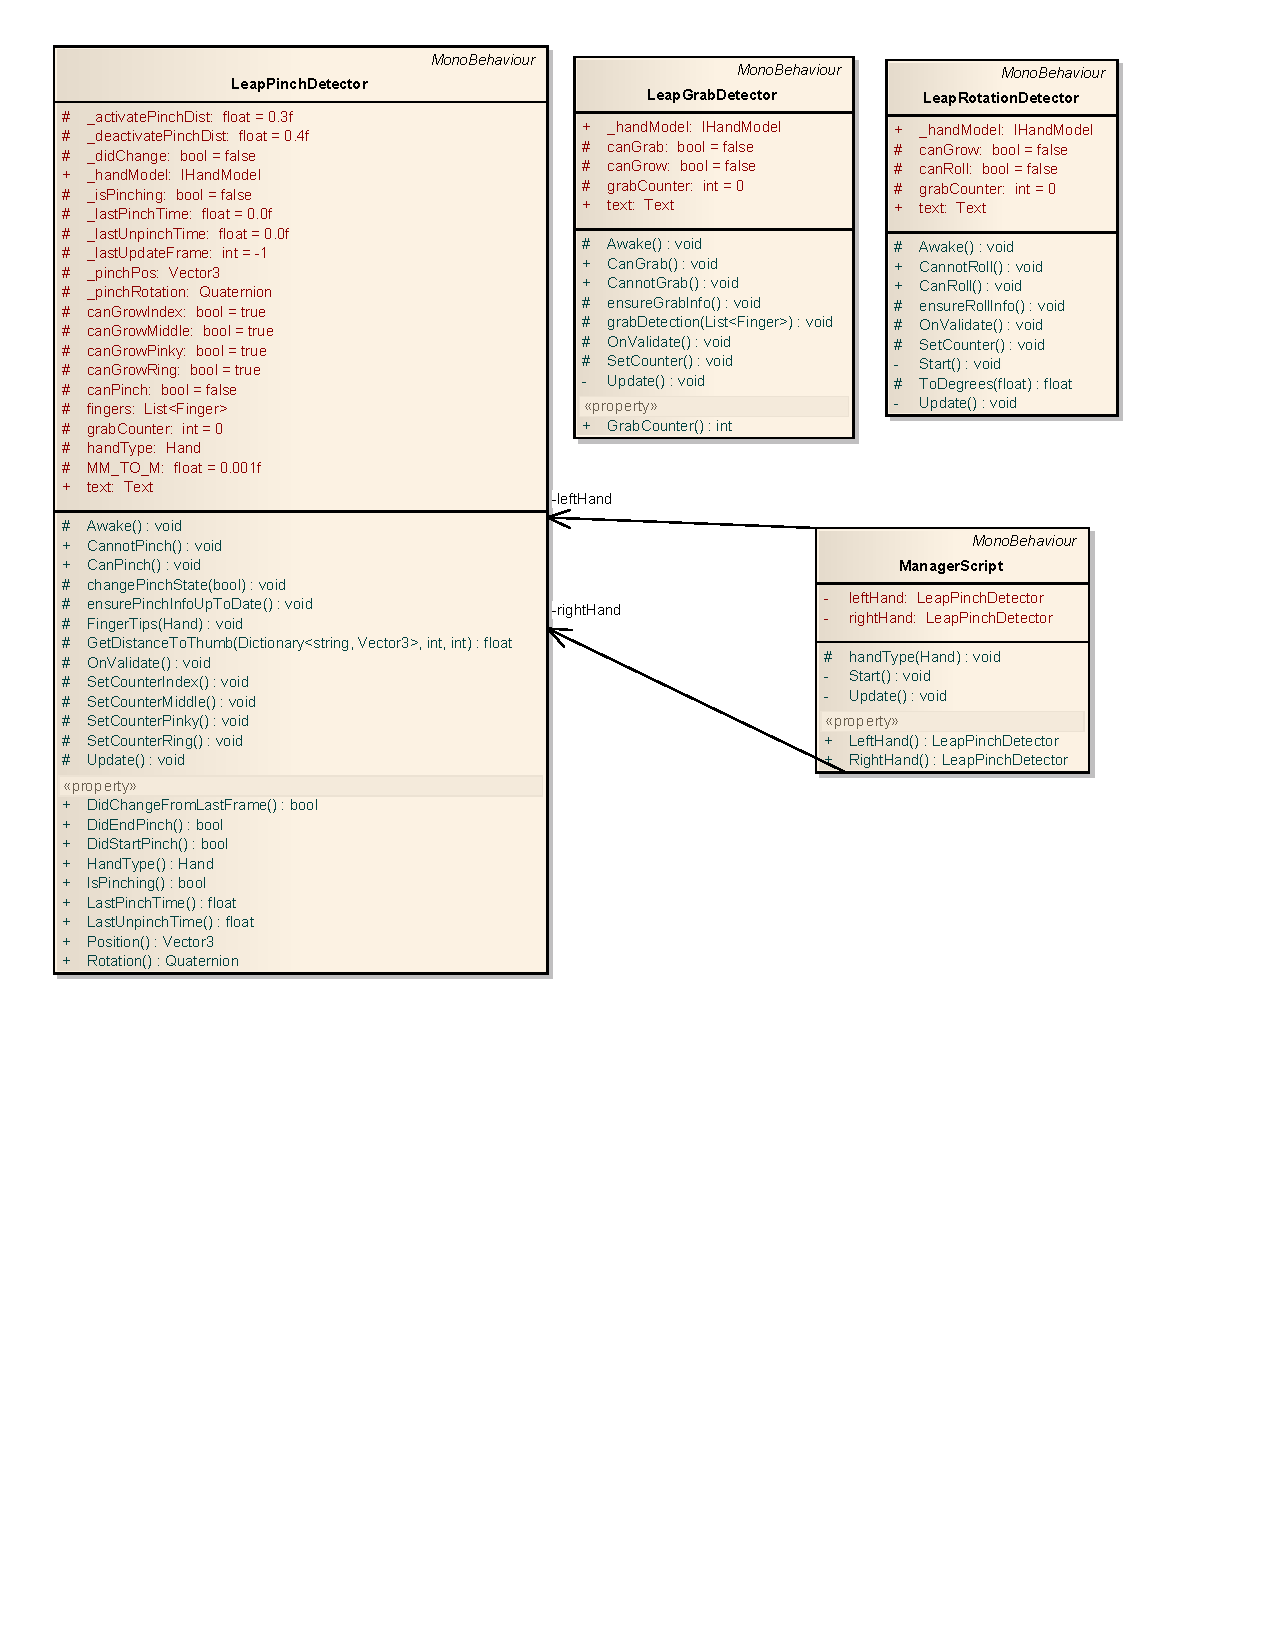
\includegraphics[trim={0 11cm 0 0.5cm},clip, width=16cm]{2_class_leapstates}
\caption{Class Diagram of Leap Motion gesture tracking.}\label{class_leap}
\end{figure}

\clearpage

\subsubsection{Sequence Diagram}
In the \mbox{figure} \ref{sequence_exercise} is represented the action of doing an exercise. In order to do that, the user must press on one of the buttons shown in the menu, after pressing one of the button, it will make a function call to the Leap Motion, by asking him to grant access on that action. The Leap Motion will send back to the user info about what button was pressed and what action the user can do now. After the user pressed on of these buttons he can do now the action itself. Also after every set of exercise in that action, the user is able to retrieve the status of his action from Leap Motion 

\begin{figure}[!h]
\centering
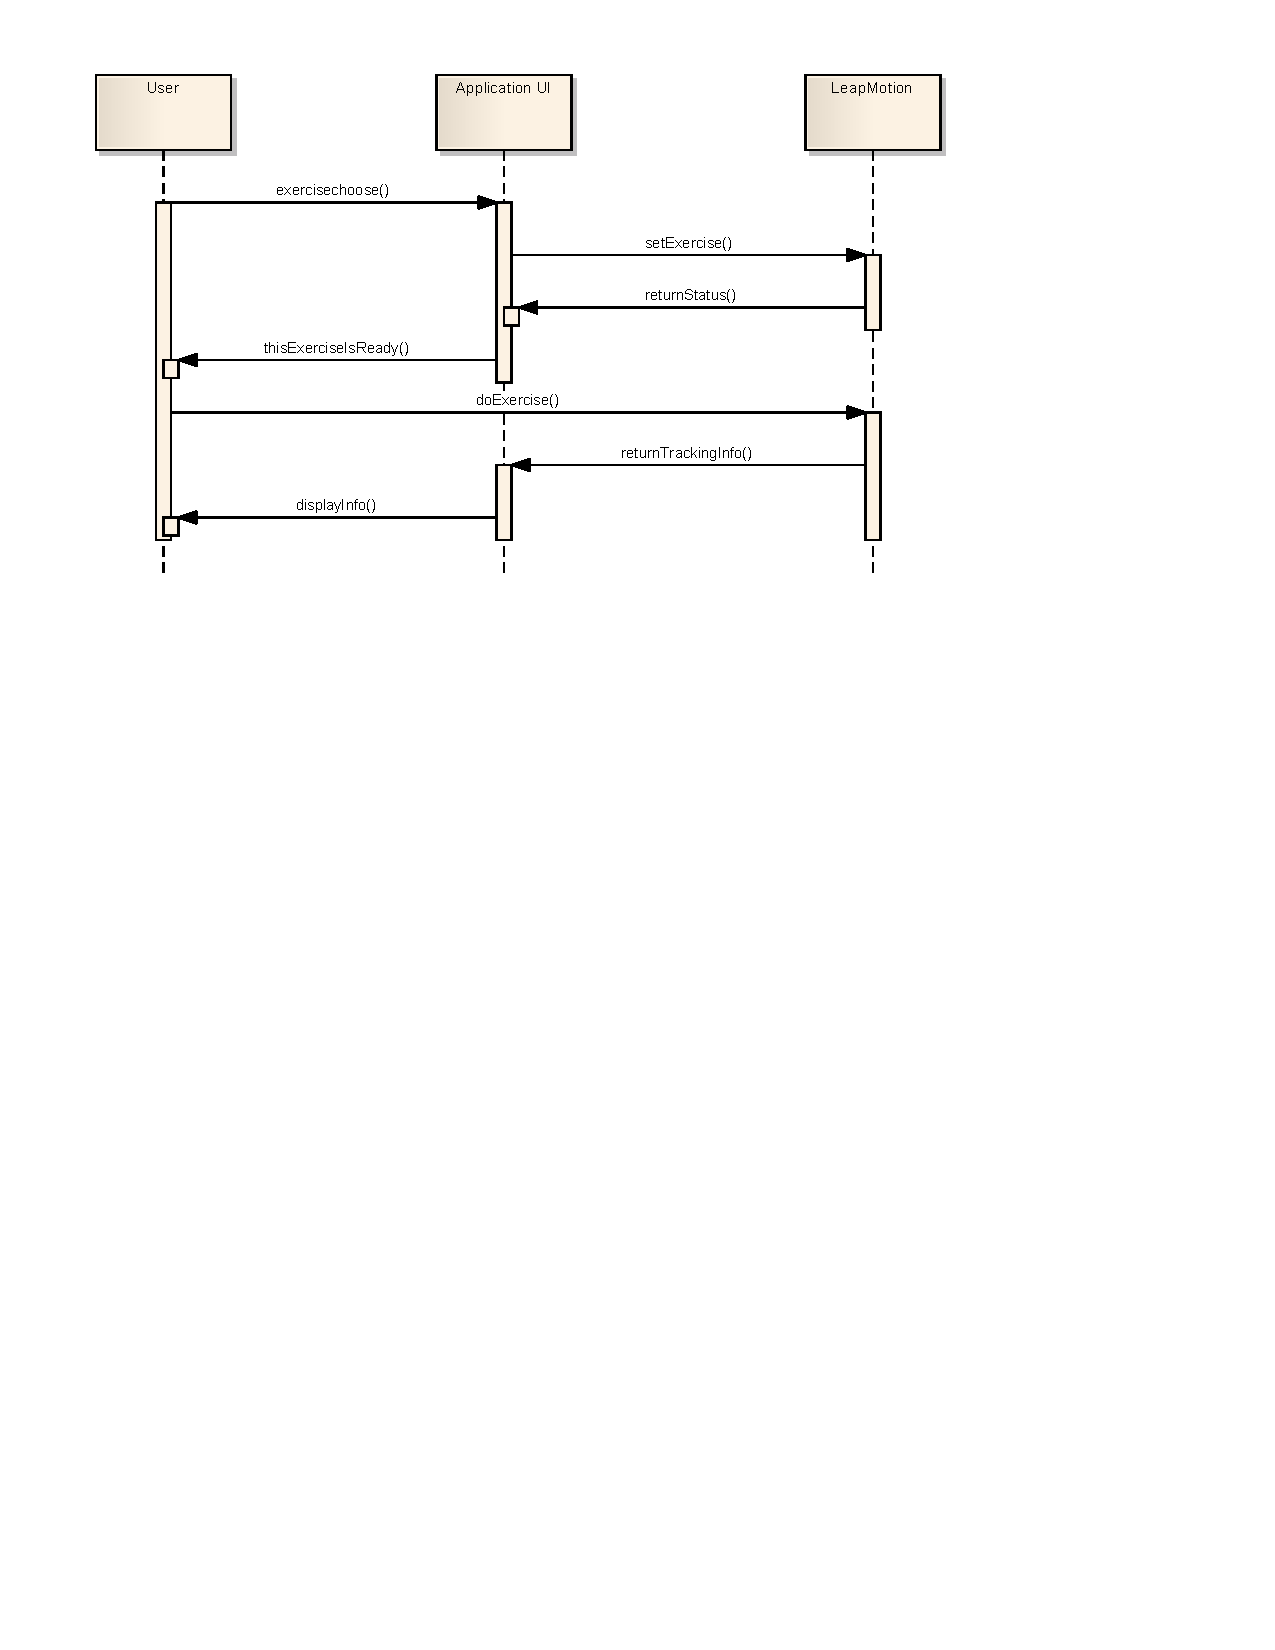
\includegraphics[trim={0 18cm 0 1cm},clip, width = 16cm]{1_sequence_exercise}
\caption{Sequence diagram of doing an exercise set.}\label{sequence_exercise}
\end{figure}
From the first glance each action behavior looks similar, having the same interface, however each has unique characteristics worth checking out. The entire process is straight and monotonous. Anyway there has to be some conditions which is the LeapMotion device is required to be connected to the users device.
\clearpage

\subsubsection{Activity Diagram}
Activity diagram is another important diagram in UML to describe dynamic aspects of the system. This diagram is basically a flow chart to represent the flow form one activity to another activity. The activity can be described as an operation of the system.

So the control flow is drawn from one operation to another. This flow can be sequential, branched or concurrent. Activity diagrams deals with all type of flow control by using different elements like fork, join etc.


Purpose of activity diagram can be:
\begin{itemize}
\item Draw the activity flow of a system.
\item Describe the sequence from one activity to another.
\item Describe the parallel, branched and concurrent flow of the system.
\end{itemize}
\vspace{0.2cm}

By now every step of exercising was particularly described.
The activity diagram from  \mbox{figure} \ref{activity_performs}, represents the list of actions done on the exercise part of the application. Every executed step in the chain  depends on the previous one.

\begin{figure}[!h]
\centering
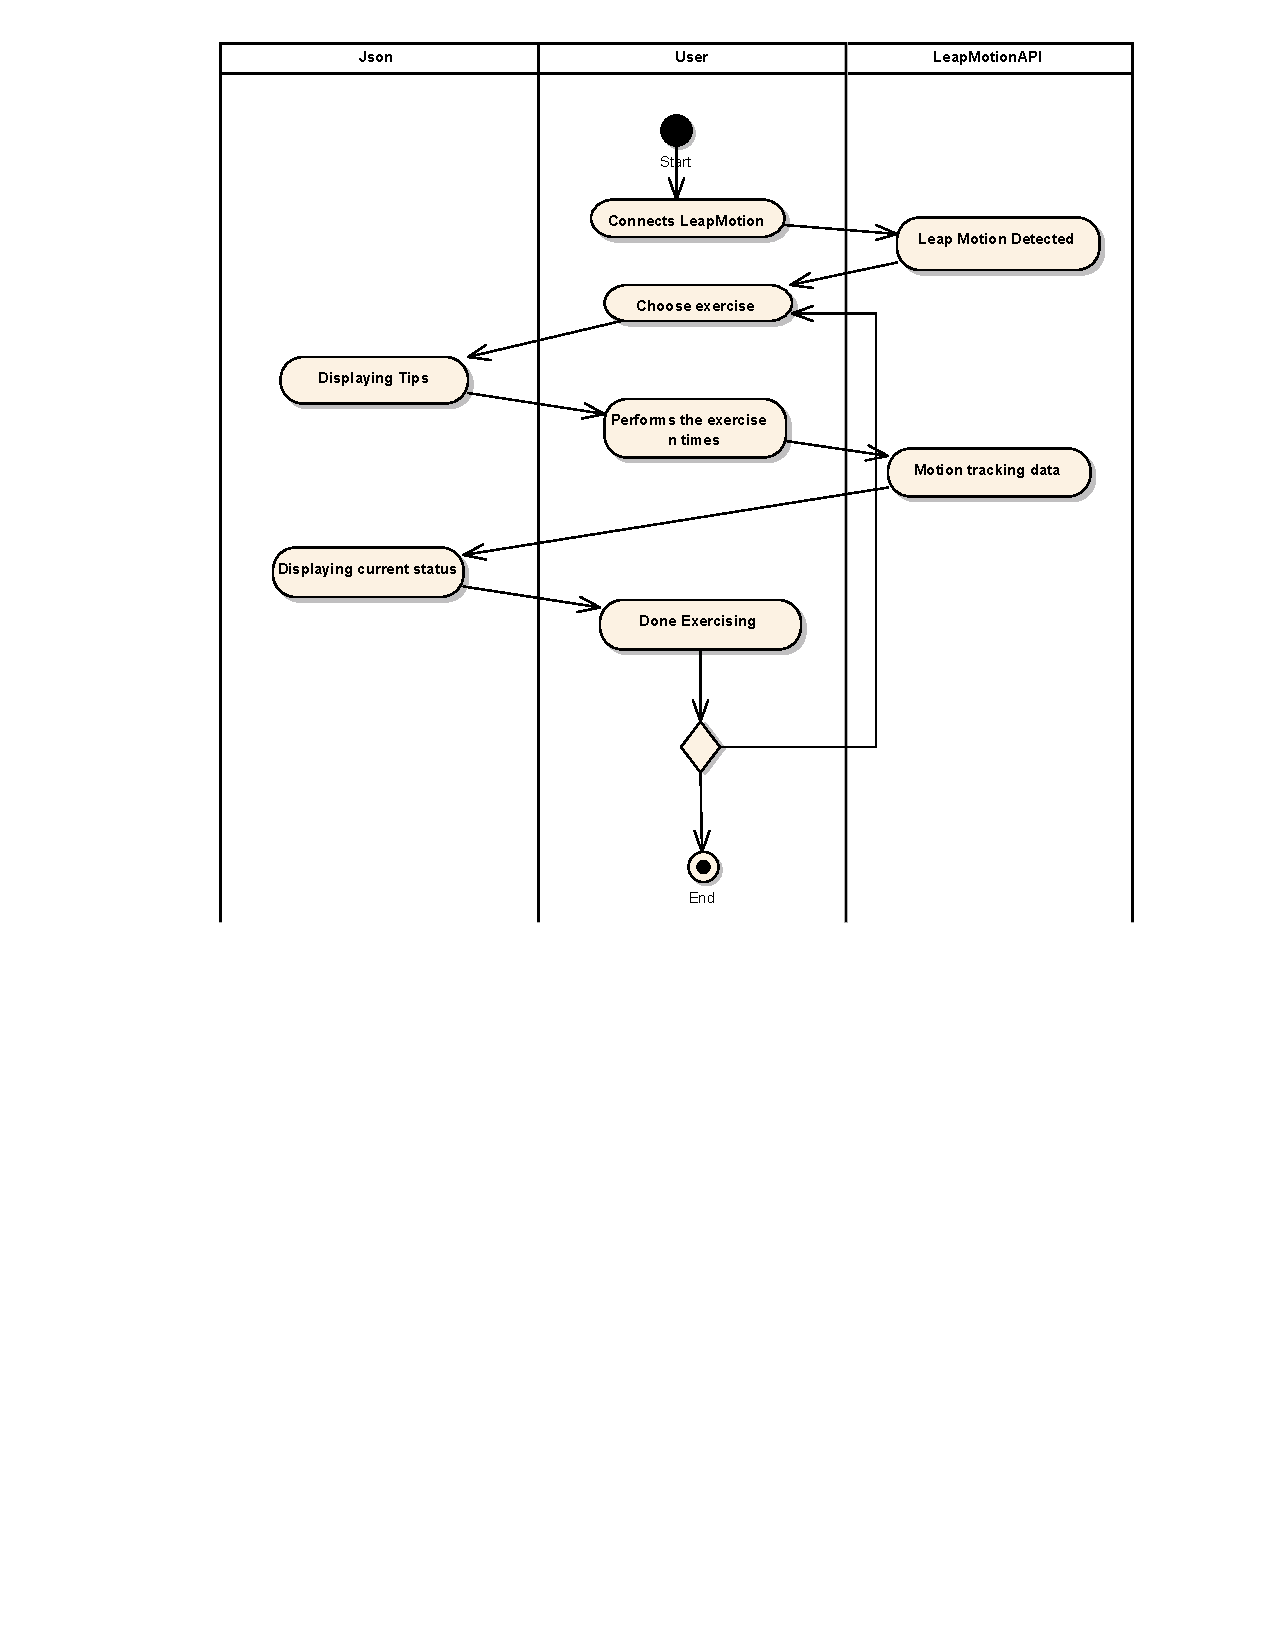
\includegraphics[trim={2cm 13cm 0 0.5cm},clip, width = 16cm]{1_activity_performs_exercise}
\caption{Exercise performing activity diagram.}\label{activity_performs}
\end{figure}

\clearpage

\subsubsection{State Diagram}
The name of the diagram itself clarifies the purpose of the diagram and other details. It describes different states of a component in a system. The states are specific to a component/object of a system.

A Statechart diagram describes a state machine. Now to clarify it state machine can be defined as a machine which defines different states of an object and these states are controlled by external or internal events.

Statechart diagrams are also used for forward and reverse engineering of a system. But the main purpose is to model reactive system.


Following are the main purposes of using Statechart diagrams:

\begin{itemize}
\item Define a state machine to model states of an object.
\item To model life time of a reactive system.
\item To model dynamic aspect of a system.
\item To describe different states of an object during its life time.
\end{itemize}

\vspace{0.2cm}

In the  \mbox{figure \ref{state_choose}} and  \mbox{figure \ref{state_perform}} is represented the application state diagram.
 However due to the fact that Kyno application offers a limited amount of operations, imply that there is a small amount of states that an application user can be. All the application states are mapped to the executable. After running the application the first step is to connect the Leap Motion device. Where in the next step the Leap Motion API detects if there is or there is not connected an Leap Motion device. On the left bottom corner of the window is rendered a pie menu that can get the user into any state of the application. The remaining states are related only to visualizing the information and the exercise action itself.


\begin{figure}[!h]
\centering
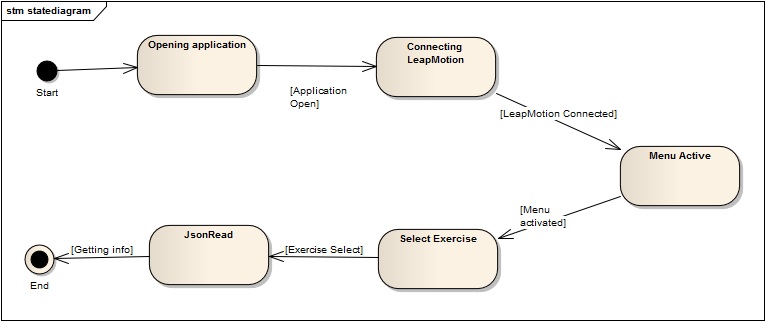
\includegraphics[trim={0 18cm 0 2cm},clip, width = 16cm]{1_state_chooseExercise}
\caption{Application state diagram.}\label{state_choose}
\end{figure}
\newpage

\begin{figure}[!h]
\centering
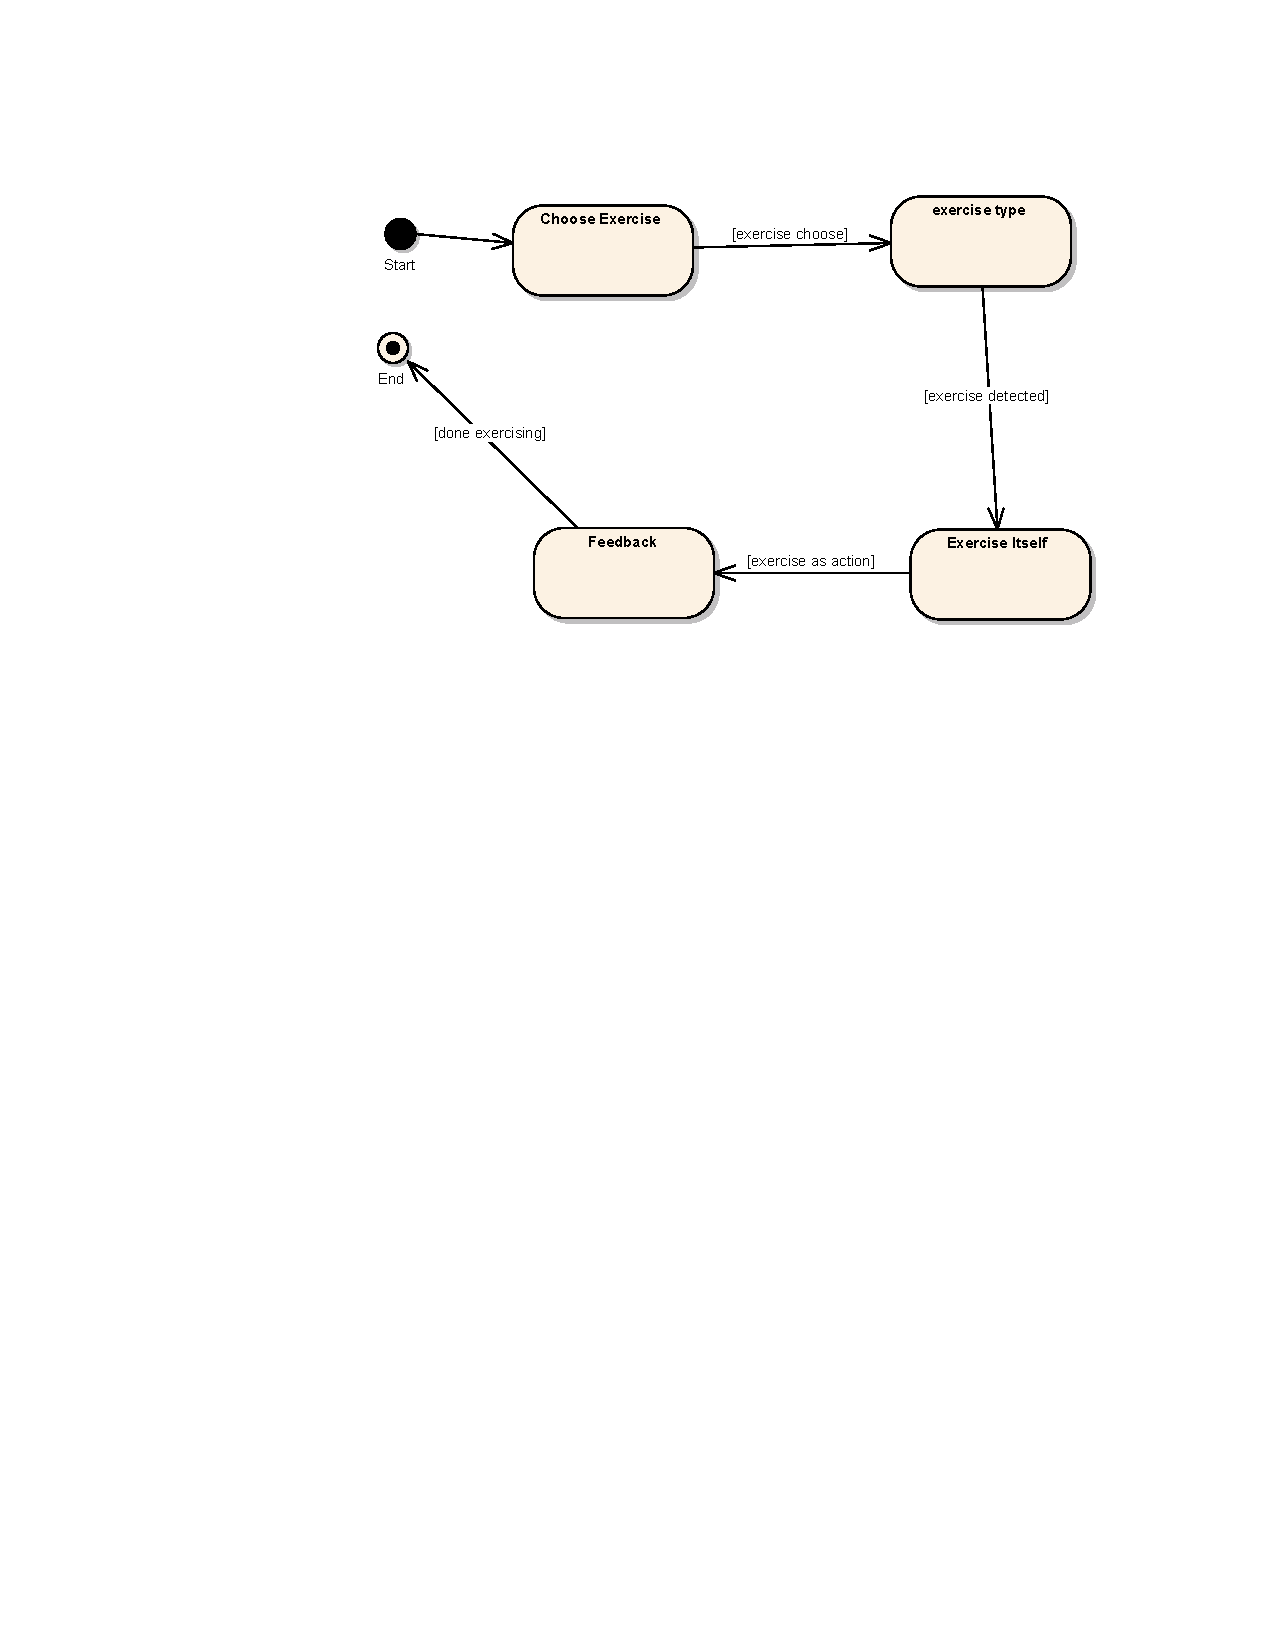
\includegraphics[trim={0 17cm 0 3cm},clip, width = 16cm]{2_state_performexercise}
\caption{Exercising state diagram}\label{state_perform}
\end{figure}



\subsection{User Experience}


\clearpage